% ====================================================================
% Appendix
% ====================================================================
\onecolumn % Switch to single-column layout
\appendix
\section{Technical Implementation Details}
\label{sec:appendix}

\subsection{Operational Traces and Log Parsing}

% --- Consolidated Figure: Standardized Height for Logs ---
\begin{figure*}[htbp]
    \centering
    \def\logheight{5.2cm} % Adjust this value to fit your page layout

    \begin{subfigure}[b]{0.32\textwidth}
        \centering
        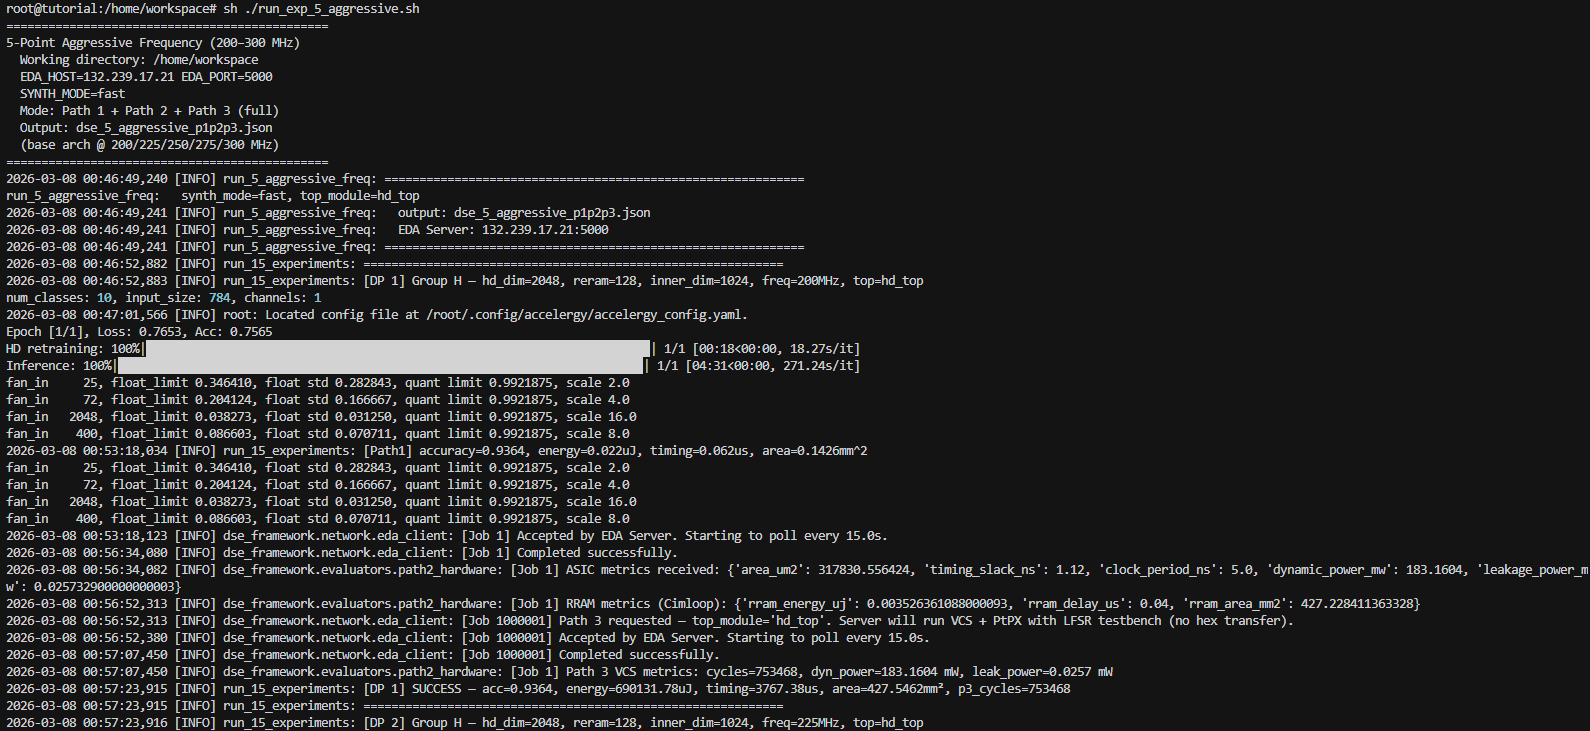
\includegraphics[width=\textwidth, height=\logheight]{images/client_full_log.png}
        \caption{Client-side orchestration.}
        \label{fig:client_log}
    \end{subfigure}
    \hfill
    \begin{subfigure}[b]{0.32\textwidth}
        \centering
        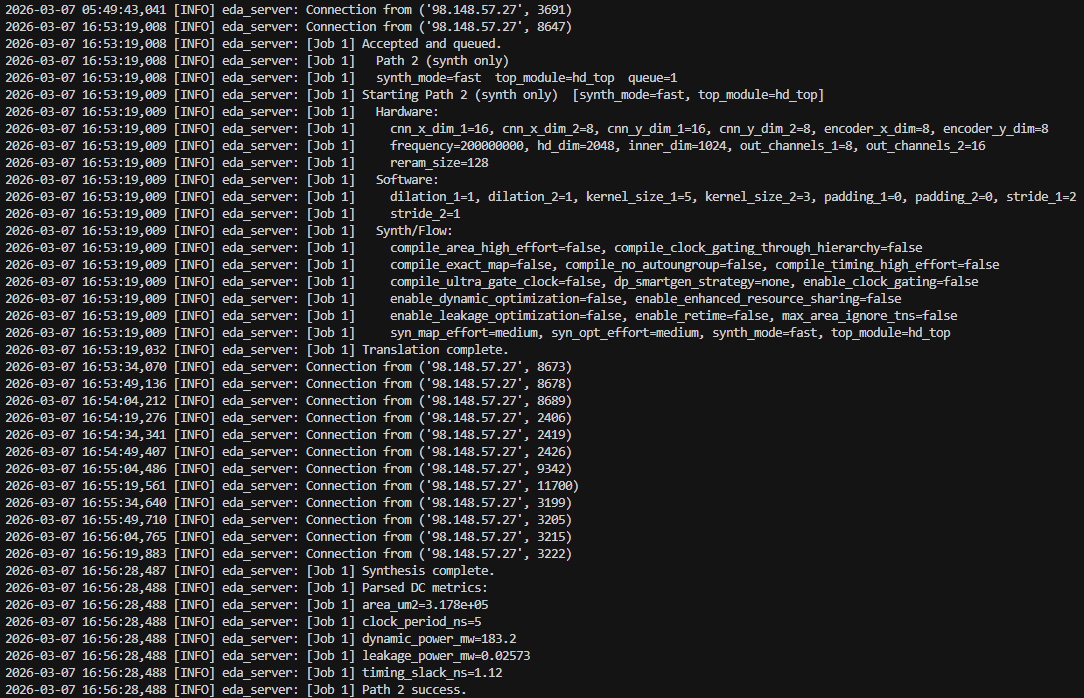
\includegraphics[width=\textwidth, height=\logheight]{images/server_path2_log.png}
        \caption{Path 2: Synthesis trace.}
        \label{fig:synthesis_log}
    \end{subfigure}
    \hfill
    \begin{subfigure}[b]{0.32\textwidth}
        \centering
        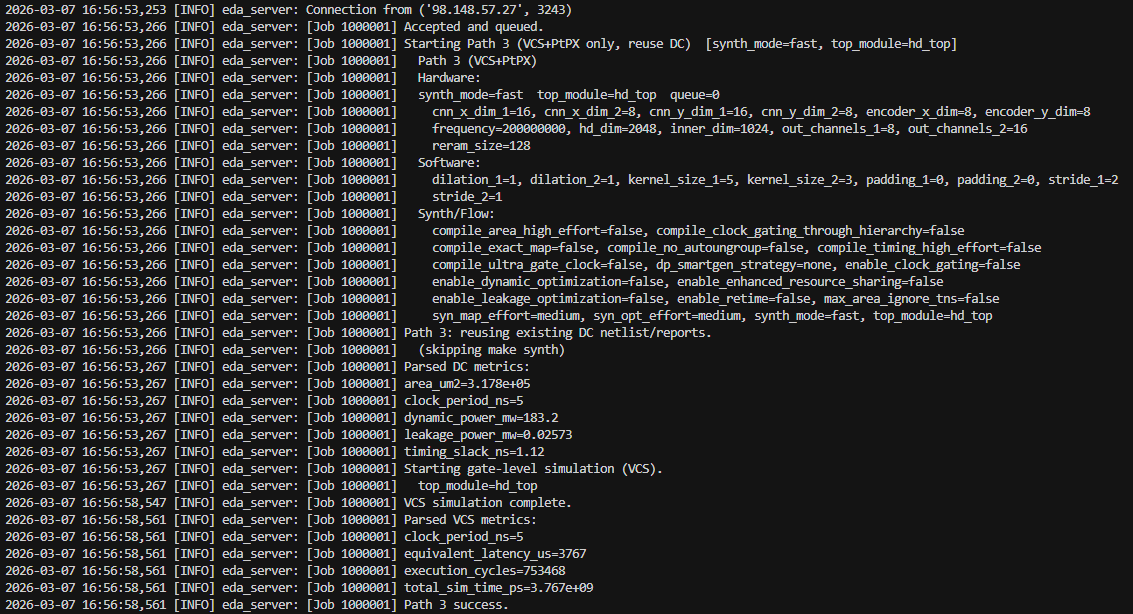
\includegraphics[width=\textwidth, height=\logheight]{images/server_path3_log.png}
        \caption{Path 3: Simulation trace.}
        \label{fig:sim_log}
    \end{subfigure}
    
    \caption{System execution traces: (a) Optimization engine managing job queues and status polling; (b) Remote server executing logic synthesis and PPA parsing; (c) High-fidelity verification highlighting waveform-driven activity monitoring.}
    \label{fig:logs}
\end{figure*}

\subsection{Hardware-Software Parameter Mapping}

% --- Table: Full-Width Parameter Mapping ---
\begin{table*}[htbp]
\centering
\caption{Cross-Layer Parameter Translation and Hardware Implementation Constraints}
\label{tab:conversion_formulas}
\begin{tabularx}{\textwidth}{@{}l l X @{}}
\toprule
\textbf{Target Primitive} & \textbf{DSE Parameter} & \textbf{Hardware Mapping Logic and Constraints} \\ \midrule
\texttt{RRAM\_ROW\_ADDR\_WIDTH} & \texttt{reram\_size} & $\lceil \log_2(\text{reram\_size}) \rceil$; must be $2^n$ for decoder. \\ \addlinespace
\texttt{HV\_LENGTH}       & \texttt{hd\_dim}     & Direct mapping; upper bound 8191 (HAMMING\_DIST\_WIDTH=13). \\ \addlinespace
\texttt{INNER\_DIM}, \texttt{WEIGHT\_MEM\_ADDR\_WIDTH} & \texttt{inner\_dim}  & $N_{\text{RF}} = \text{inner\_dim} / 32$; $W = \lceil \log_2(N_{\text{RF}}) \rceil$. \\ \addlinespace
\texttt{CNN1\_INPUTS\_NUM} & \texttt{cnn\_x\_dim\_1} $\times$ \texttt{cnn\_y\_dim\_1} & Scalar product. \\ \addlinespace
\texttt{CNN2\_INPUTS\_NUM} & \texttt{cnn\_x\_dim\_2} $\times$ \texttt{cnn\_y\_dim\_2} & Scalar product. \\ \addlinespace
\texttt{ENC\_INPUTS\_NUM} & \texttt{encoder\_x\_dim} $\times$ \texttt{encoder\_y\_dim} & Product; encoder receptive field. \\ \addlinespace
\texttt{HV\_SEG\_WIDTH} & \texttt{hd\_dim} / \texttt{ENC\_INPUTS\_NUM} & Must divide; HV\_SEG\_WIDTH $\geq$ 20; 256 mod HV\_SEG\_WIDTH = 0. \\ \addlinespace
\texttt{TB\_CLK\_PERIOD\_NS} & \texttt{frequency}   & Same; for LFSR testbench clock generator. \\ \addlinespace
\texttt{ELABORATE\_ROOT}  & \texttt{top\_module} & core or hd\_top; selects testbench. \\ \bottomrule
\end{tabularx}
\end{table*}

\subsection{Synthesis Optimization Space}
% --- Table: Full-Width Synthesis Flags ---
\begin{table*}[htbp]
\centering
\caption{Definitions of Fine-Grained Synthesis Flags and Mapping to EDA Directives}
\label{tab:synthesis_flags}
\begin{tabularx}{\textwidth}{@{}l l X @{}}
\toprule
\textbf{DSE Control Knob} & \textbf{Data Type} & \textbf{Target Design Compiler (DC) Implementation Directive} \\ \midrule
\texttt{enable\_clock\_gating} & Boolean & \texttt{set\_clock\_gating\_style} -sequential\_cell latch + \texttt{insert\_clock\_gating} \\ \addlinespace
\texttt{max\_area\_ignore\_tns} & Boolean & \texttt{set\_max\_area 0 -ignore\_tns} (area over TNS). \\ \addlinespace
\texttt{enable\_retime}        & Boolean & \texttt{compile\_ultra -retime} \\ \addlinespace
\texttt{compile\_timing\_high\_effort}  & Boolean & \texttt{compile\_ultra -timing\_high\_effort\_script} \\ \addlinespace
\texttt{compile\_area\_high\_effort}    & Boolean & \texttt{compile\_ultra -area\_high\_effort\_script} \\ \addlinespace
\texttt{compile\_ultra\_gate\_clock}    & Boolean & \texttt{compile\_ultra -gate\_clock} \\ \addlinespace
\texttt{compile\_exact\_map}            & Boolean & \texttt{compile\_ultra -exact\_map} \\ \addlinespace
\texttt{compile\_no\_autoungroup}       & Boolean & \texttt{compile\_ultra -no\_autoungroup} \\ \addlinespace
\texttt{compile\_clock\_gating\_through\_hierarchy} & Boolean & \texttt{set compile\_clock\_gating\_through\_hierarchy true} \\ \addlinespace
\texttt{enable\_leakage\_optimization} & Boolean & \texttt{set\_leakage\_optimization true} \\ \addlinespace
\texttt{enable\_dynamic\_optimization} & Boolean & \texttt{set\_dynamic\_optimization true} \\ \addlinespace
\texttt{enable\_enhanced\_resource\_sharing} & Boolean & \texttt{set compile\_enhanced\_resource\_sharing true} \\ \addlinespace
\texttt{dp\_smartgen\_strategy} & Categorical & \texttt{set\_dp\_smartgen\_options -optimization\_strategy} [timing|area] \\ \bottomrule
\end{tabularx}
\end{table*}